% -----------------------------*- LaTeX -*------------------------------
\documentclass[UTF8]{report}
% ------------------------------------------------------------------------
% Packages
% ------------------------------------------------------------------------
\usepackage{ctex} % 支持中文
\usepackage[body={7in, 9in},left=1in,right=1in]{geometry} % 改变页边距
\usepackage{amsmath} % AMS 的数学宏包
\usepackage{amsfonts} % AMS 的数学字体宏包
\usepackage{amssymb} % AMS 符号库
\usepackage{bm} % 数学公式中的黑斜体
\usepackage{amsthm} % AMS 的定理环境宏包
\usepackage{graphicx} % 插图
\usepackage{subfigure} % 插子图
\usepackage{nicefrac} % 好看的分数
\usepackage{mathrsfs} % mathscr font
\usepackage{caption} % caption
\usepackage{algorithm,algorithmicx} % 伪代码支持宏包
\usepackage[noend]{algpseudocode} % 伪代码
\usepackage{fancyhdr} % 设置页眉、页脚
\usepackage{adjustbox} % 图片尺寸自动调整
\usepackage{esint} % 积分符号
\usepackage{mathtools} % 数学宏包的重要补充
\usepackage{upgreek} % 数学环境的直立希腊字母
\usepackage{enumitem} % 使用enumitem宏包, 改变列表项的格式
\usepackage{color} % 支持彩色
\usepackage{extarrows} % 任意长度的箭头
\usepackage{tikz} % 绘图
\usepackage{forest} % 绘树
\usepackage{xcolor} % 颜色宏包
\usepackage{breqn} % 公式自动换行
\usepackage{fontsize} % 字体大小
\usepackage[framemethod=TikZ]{mdframed} % 给文字加框
\usepackage{fontspec} % 字体库
\usepackage{bigstrut} % 用于表格中的换行
\usepackage{multirow} % 表格中多行单元格合并
\usepackage{multicol} % 表格中多列单元格合并
\usepackage{longtable} % 长表格
\usepackage{rotating} % 旋转图形和表格      以上三者用于绘制三线表
\usepackage{booktabs} % 三线表宏包
\usepackage{scribe} % Scribe 模板
\usepackage{diagbox} % 表格斜线
\usepackage{listings} % 插入代码
\usepackage{verbatim} % 多行注释
\usepackage{ifplatform} % 检测编译平台
\usepackage{pifont} % 圆圈数字
\usetikzlibrary{shapes.geometric, arrows} % 引入流程图需要的库
\usetikzlibrary{automata} % 引入automata库
\usetikzlibrary{shapes,arrows,positioning,chains} % 引入positioning库
% ------------------------------------------------------------------------
% Macros
% ------------------------------------------------------------------------
%~~~~~~~~~~~~~~~
% Utility latin
%~~~~~~~~~~~~~~~
\newcommand{\ie}{\textit{i.e.}}
\newcommand{\eg}{\textit{e.g.}}
%~~~~~~~~~~~~~~~
% Environment shortcuts
%~~~~~~~~~~~~~~~
\newcommand{\balign}[1]{\ealign{\begin{align}#1\end{align}}}
\newcommand{\baligns}[1]{\ealigns{\begin{align*}#1\end{align*}}}
\newcommand{\bitemize}[1]{\eitemize{\begin{itemize}#1\end{itemize}}}
\newcommand{\benumerate}[1]{\eenumerate{\begin{enumerate}#1\end{enumerate}}}
%~~~~~~~~~~~~~~~
% Text with quads around it
%~~~~~~~~~~~~~~~
\newcommand{\qtext}[1]{\quad\text{#1}\quad}
%~~~~~~~~~~~~~~~
% Shorthand for math formatting
%~~~~~~~~~~~~~~~
\newcommand{\mbb}[1]{\mathbb{#1}}
\newcommand{\mbi}[1]{\boldsymbol{#1}} % Bold and italic (math bold italic)
\newcommand{\mbf}[1]{\mathbf{#1}}
\newcommand{\mc}[1]{\mathcal{#1}}
\newcommand{\mrm}[1]{\mathrm{#1}}
\newcommand{\tbf}[1]{\textbf{#1}}
\newcommand{\tsc}[1]{\textsc{#1}}
%\def\\langle {{\langle }}
%\def\\rangle {{\rangle }}
\newcommand{\sT}{\sf T}
\newcommand{\grad}{\nabla}
\newcommand{\Proj}{\Pi}
%~~~~~~~~~~~~~~~
% Common sets 定义数集符号
%~~~~~~~~~~~~~~~
\newcommand{\R}{\mathbb{R}}
\newcommand{\Z}{\mathbb{Z}}
\newcommand{\Q}{\mathbb{Q}}
\newcommand{\N}{\mathbb{N}}
\newcommand{\C}{\mathbb{C}}
\newcommand{\reals}{\mathbb{R}} % Real number symbol
\newcommand{\integers}{\mathbb{Z}} % Integer symbol
\newcommand{\rationals}{\mathbb{Q}} % Rational numbers
\newcommand{\naturals}{\mathbb{N}} % Natural numbers
\newcommand{\complex}{\mathbb{C}} % Complex numbers
%~~~~~~~~~~~~~~~
% Common functions
%~~~~~~~~~~~~~~~
\renewcommand{\exp}[1]{\operatorname{exp}\left(#1\right)} % Exponential
\newcommand{\indic}[1]{\mbb{I}\left(#1\right)} % Indicator function
\newcommand{\indicsub}[2]{\mbb{I}_{#2}\left(#1\right)} % Indicator function
\newcommand{\argmax}{\mathop\mathrm{arg\, max}} % Defining math symbols
\newcommand{\argmin}{\mathop\mathrm{arg\, min}}
\renewcommand{\arccos}{\mathop\mathrm{arccos}}
\newcommand{\dom}{\mathop\mathrm{dom}} % Domain
\newcommand{\range}{\mathop\mathrm{range}} % Range
\newcommand{\diag}{\mathop\mathrm{diag}}
\newcommand{\tr}{\mathop\mathrm{tr}}
\newcommand{\abs}{\mathop\mathrm{abs}}
\newcommand{\card}{\mathop\mathrm{card}}
\newcommand{\sign}{\mathop\mathrm{sign}}
\newcommand{\prox}{\mathrm{prox}} % prox
\newcommand{\rank}[1]{\mathrm{rank}(#1)}
\newcommand{\supp}[1]{\mathrm{supp}(#1)}
\newcommand{\norm}[1]{\lVert#1\rVert}
%~~~~~~~~~~~~~~~
% Common probability symbols
%~~~~~~~~~~~~~~~
\newcommand{\family}{\mathcal{P}} % probability family / statistical model
\newcommand{\iid}{\stackrel{\mathrm{iid}}{\sim}}
\newcommand{\ind}{\stackrel{\mathrm{ind}}{\sim}}
\newcommand{\E}{\mathbb{E}} % Expectation symbol
\newcommand{\Earg}[1]{\E\left[#1\right]}
\newcommand{\Esubarg}[2]{\E_{#1}\left[#2\right]}
\renewcommand{\P}{\mathbb{P}} % Probability symbol
\newcommand{\Parg}[1]{\P\left(#1\right)}
\newcommand{\Psubarg}[2]{\P_{#1}\left[#2\right]}
%\newcommand{\Cov}{\mrm{Cov}} % Covariance symbol
%\newcommand{\Covarg}[1]{\Cov\left[#1\right]}
%\newcommand{\Covsubarg}[2]{\Cov_{#1}\left[#2\right]}
%\newcommand{\model}{\mathcal{P}} % probability family / statistical model
%~~~~~~~~~~~~~~~
% Distributions
%~~~~~~~~~~~~~~~
%\newcommand{\Gsn}{\mathcal{N}}
%\newcommand{\Ber}{\textnormal{Ber}}
%\newcommand{\Bin}{\textnormal{Bin}}
%\newcommand{\Unif}{\textnormal{Unif}}
%\newcommand{\Mult}{\textnormal{Mult}}
%\newcommand{\NegMult}{\textnormal{NegMult}}
%\newcommand{\Dir}{\textnormal{Dir}}
%\newcommand{\Bet}{\textnormal{Beta}}
%\newcommand{\Gam}{\textnormal{Gamma}}
%\newcommand{\Poi}{\textnormal{Poi}}
%\newcommand{\HypGeo}{\textnormal{HypGeo}}
%\newcommand{\GEM}{\textnormal{GEM}}
%\newcommand{\BP}{\textnormal{BP}}
%\newcommand{\DP}{\textnormal{DP}}
%\newcommand{\BeP}{\textnormal{BeP}}
%\newcommand{\Exp}{\textnormal{Exp}}
%~~~~~~~~~~~~~~~
% Theorem-like environments
%~~~~~~~~~~~~~~~
%\theoremstyle{definition}
%\newtheorem{definition}{Definition}
%\newtheorem{example}{Example}
%\newtheorem{problem}{Problem}
%\newtheorem{lemma}{Lemma}
%~~~~~~~~~~~~~~~
% 组合数学的模板和作业里用到的一些宏包和自定义命令
%~~~~~~~~~~~~~~~
\renewcommand{\emph}[1]{\begin{kaishu}#1\end{kaishu}}
\newcommand{\falfac}[1]{^{\underline{#1}}}
\newcommand{\binomfrac}[2]{\frac{#1^{\underline{#2}}}{#2!}}
\newcommand{\ceil}[1]{\left\lceil #1 \right\rceil}
\newcommand{\floor}[1]{\left\lfloor #1 \right\rfloor}
\newcommand{\suminfty}[2]{\sum_{#1=#2}^{\infty}}
\newcommand{\suminftyk}[0]{\sum_{k=0}^{\infty}}
\newcommand{\sumint}[3]{\sum_{#1=#2}^{#3}}
\newcommand{\sumintk}[2]{\sum_{k=#1}^{#2}}
\newcommand{\suminti}[2]{\sum_{i=#1}^{#2}}
%~~~~~~~~~~~~~~~
% 定义新命令
%~~~~~~~~~~~~~~~
\newcommand*{\unit}[1]{\mathop{}\!\mathrm{#1}}
\newcommand*{\dif}{\mathop{}\!\mathrm{d}}%微分算子 d
\newcommand*{\pdif}{\mathop{}\!\partial}%偏微分算子
\newcommand*{\cdif}{\mathop{}\!\nabla}%协变导数、nabla 算子
\newcommand*{\laplace}{\mathop{}\!\Delta}%laplace 算子
\newcommand*{\deri}[1]{\mathrm{d} #1}
\newcommand*{\deriv}[2]{\frac{\mathrm{d} #1}{\mathrm{d} {#2}}}
\newcommand*{\derivh}[3]{\frac{\mathrm{d}^{#1} #2}{\mathrm{d} {#3^{#1}}}}
\newcommand*{\pderiv}[2]{\frac{\partial #1}{\partial {#2}}}
\newcommand*{\pderivh}[3]{\frac{\partial^{#1} #2}{\partial {#3^{#1}}}}
\newcommand*{\dderiv}[2]{\dfrac{\mathrm{d} #1}{\mathrm{d} {#2}}}
\newcommand*{\dderivh}[3]{\dfrac{\mathrm{d}^{#1} #2}{\mathrm{d} {#3^{#1}}}}
\newcommand*{\dpderiv}[2]{\dfrac{\partial #1}{\partial {#2}}}
\newcommand*{\dpderivh}[3]{\dfrac{\partial^{#1} #2}{\partial {#3^{#1}}}}
\newcommand{\me}[1]{\mathrm{e}^{#1}}%e 指数
\newcommand{\mi}{\mathrm{i}}%虚数单位
%\newcommand{\mc}{\mathrm{c}}%光速 定义与mathcal冲突
\newcommand{\red}[1]{\textcolor{red}{#1}}
\newcommand{\blue}[1]{\textcolor{blue}{#1}}
%\newcommand{\Rome}[1]{\setcounter{rome}{#1}\Roman{rome}}
%~~~~~~~~~~~~~~~
% 公式环境中箭头符号的简写
%~~~~~~~~~~~~~~~
\newcommand{\ra}{\rightarrow}
\newcommand{\Ra}{\Rightarrow}
\newcommand{\la}{\leftarrow}
\newcommand{\La}{\Leftarrow}
\newcommand{\lra}{\leftrightarrow}
\newcommand{\Lra}{\Leftrightarrow}
\newcommand{\lgla}{\longleftarrow}
\newcommand{\Lgla}{\Longleftarrow}
\newcommand{\lgra}{\longrightarrow}
\newcommand{\Lgra}{\Longrightarrow}
\newcommand{\lglra}{\longleftrightarrow}
\newcommand{\Lglra}{\Longleftrightarrow}
%~~~~~~~~~~~~~~~
% 一些数学的环境设置
%~~~~~~~~~~~~~~~
%\newcounter{counter_exm}\setcounter{counter_exm}{1}
%\newcounter{counter_prb}\setcounter{counter_prb}{1}
%\newcounter{counter_thm}\setcounter{counter_thm}{1}
%\newcounter{counter_lma}\setcounter{counter_lma}{1}
%\newcounter{counter_dft}\setcounter{counter_dft}{1}
%\newcounter{counter_clm}\setcounter{counter_clm}{1}
%\newcounter{counter_cly}\setcounter{counter_cly}{1}
\newtheorem{theorem}{{\hskip 1.7em \bf 定理}}
\newtheorem{lemma}[theorem]{\hskip 1.7em 引理}
\newtheorem{proposition}[theorem]{\hskip 1.7em 命题}
\newtheorem{claim}[theorem]{\hskip 1.7em 断言}
\newtheorem{corollary}[theorem]{\hskip 1.7em 推论}
% \newcommand{\problem}[1]{{\setlength{\parskip}{10pt}\noindent \bf{#1}}}
\newenvironment{solution}{{\noindent \bf 解 \quad}}{}
\newenvironment{remark}{{\noindent \bf 注 \quad}}{}
\newenvironment{definition}{{\noindent \bf 定义 \quad}}{}
\renewenvironment{proof}{{\setlength{\parskip}{7pt}\noindent\hskip 2em \bf 证明 \quad}}{\hfill$\qed$\par}
\newenvironment{example}{{\noindent\bf 例 \quad}}{\hfill$\qed$\par}
%\newenvironment{concept}[1]{{\bf #1\quad} \begin{kaishu}} {\end{kaishu}\par}
%~~~~~~~~~~~~~~~
% 本.tex文档中特殊定义命令
%~~~~~~~~~~~~~~~
\newcommand{\lno}[1]{\overline{#1}}
\newcommand{\NP}{\mathrm{NP}}
\newcommand{\coNP}{\mathrm{coNP}}
% \newcommand{\ISO}{\mathrm{ISO}}
\newcommand{\SAT}{\mathrm{SAT}}
\newcommand{\USAT}{\mathrm{USAT}}
% \newcommand{\threeSAT}{\mathrm{3\text{-}SAT}}
\renewcommand{\P}{\mathrm{P}}
% \mathchardef\mhyphen="2D
% \newcommand{\CNF}{\mathrm{CNF}}
% \newcommand{\DNF}{\mathrm{DNF}}
% \newcommand{\SetSp}{\mathrm{SET\text{-}SPLITTING}}
% \newcommand{\PUZZLE}{\mathrm{PUZZLE}}
% \newcommand{\SPATH}{\mathrm{SPATH}}
% \newcommand{\LPATH}{\mathrm{LPATH}}
% \newcommand{\UHAMPATH}{\mathrm{UHAMPATH}}
\newcommand{\SPACE}{\mathrm{SPACE}}
\newcommand{\NSPACE}{\mathrm{NSPACE}}
\newcommand{\PSPACE}{\mathrm{PSPACE}}
\newcommand{\NPSPACE}{\mathrm{NPSPACE}}
\newcommand{\DFA}{\mathrm{DFA}}
\newcommand{\NFA}{\mathrm{NFA}}
\newcommand{\TQBF}{\mathrm{TQBF}}
% \newcommand{\L}{\mathrm{L}}
\renewcommand{\O}{\mathrm{O}}
\newcommand{\NL}{\mathrm{NL}}
\newcommand{\coNL}{\mathrm{coNL}}
\newcommand{\LADDER}{\mathrm{LADDER_{DFA}}}
\newcommand{\hd}{\mathrm{\text{-}hard}}
\newcommand{\ADD}{\mathrm{ADD}}
\newcommand{\STCN}{\mathrm{STRONGLY\text{-}CONNECTED}}
\newcommand{\PATH}{\mathrm{PATH}}
\newcommand{\A}{\mathrm{A}}
%使用align环境公式换页
\allowdisplaybreaks[4]

\definecolor{dkgreen}{rgb}{0,0.6,0}
\definecolor{gray}{rgb}{0.5,0.5,0.5}
\definecolor{mauve}{rgb}{0.58,0,0.82}
\lstset{
  frame=tb,
  aboveskip=3mm,
  belowskip=3mm,
  showstringspaces=false,
  columns=flexible,
  framerule=1pt,
  rulecolor=\color{gray!35},
  backgroundcolor=\color{gray!5},
  basicstyle={\small\ttfamily},
  numbers=none,
  numberstyle=\tiny\color{gray},
  keywordstyle=\color{blue},
  commentstyle=\color{dkgreen},
  stringstyle=\color{mauve},
  breaklines=true,
  breakatwhitespace=true,
  tabsize=3,
}

\tikzstyle{startstop} = [rectangle, rounded corners, minimum width=3cm, minimum height=1cm,text centered, draw=black, fill=red!30]
\tikzstyle{process} = [rectangle, minimum width=3cm, minimum height=1cm, text centered, draw=black, fill=orange!30]
\tikzstyle{decision} = [diamond, minimum width=3cm, minimum height=1cm, text centered, draw=black, fill=green!30]
\tikzstyle{arrow} = [thick,->,>=stealth]

\ifwindows
    \setmainfont{Times New Roman}
    \setsansfont{Times New Roman}
    \setmonofont{Consolas}
    \setCJKmainfont{SimHei}
    \setCJKsansfont{SimSun}
    \setCJKmonofont{FangSong}
\fi

\ifmacosx
    \setmainfont{Times New Roman}
    \setsansfont{Times New Roman}
    \setmonofont{Menlo}
    \setCJKmainfont{STHeiti}
    \setCJKsansfont{STSong}
    \setCJKmonofont{STFangsong}
\fi

\punctstyle{kaiming}

\begin{document}

\pagestyle{fancy}

\reporttype{Report}                 % required
\course{Lab of Computer Network} 				% optional
\coursetitle{Router}	    % optional
\semester{Fall 2024}			    % optional
\lecturer{Wu Qinghua}			% optional
\scribe{2022K8009929010 Zhang Jiawei}			% required
\lecturenumber{7}				% required (must be a number)
\lecturedate{October 29}			% required (omit year)
\maketitle

\section{实验内容}

\begin{enumerate}
    \item 
    \begin{enumerate}
        \item 在主机上安装arptables, iptables,用于禁止每个节点的相应功能。
        \item 运行给定网络拓扑:路由器节点r1上执行脚本(disable_arp.sh, disable_icmp.sh, disable_ip_forward.sh),禁止协议栈的相应功能;终端节点h1-h3上执行脚本disable_offloading.sh。
        \item 在r1上执行路由器程序。
        \item 在h1上进行ping实验:Ping 10.0.1.1 (r1),能够ping通;Ping 10.0.2.22 (h2),能够ping通;Ping 10.0.3.33 (h3),能够ping通;Ping 10.0.3.11,返回ICMP Destination Host Unreachable;Ping 10.0.4.1,返回ICMP Destination Net Unreachable。
    \end{enumerate}
    \item 
    \begin{enumerate}
        \item 构造一个包含多个路由器节点组成的网络:手动配置每个路由器节点的路由表;有两个终端节点,通过路由器节点相连,两节点之间的跳数不少于3跳,手动配置其默认路由表。
        \item 连通性测试:终端节点ping每个路由器节点的入端口IP地址,能够ping通。
        \item 路径测试:在一个终端节点上traceroute另一节点,能够正确输出路径上每个节点的IP信息。
    \end{enumerate}
\end{enumerate}

\section{实验过程}

\subsection{IP数据包转发}

对于路由器接收到的IP报文,在转发之前需要先进行一次判定。倘若该报文为ICMP协议下的请求回复报文(\texttt{ICMP_ECHOREQUEST})且目的地址为路由器的入端口IP地址,直接向源地址发送ICMP回复报文(\texttt{ICMP_ECHOREPLY}):

\begin{lstlisting}[language=C]
	struct iphdr *iphdr = packet_to_ip_hdr(packet);
	struct icmphdr *icmphdr = (struct icmphdr *)IP_DATA(iphdr);
	u32 dest = ntohl(iphdr->daddr);
	u8 protocol = iphdr->protocol;
	u8 type = icmphdr->type;

	// check if the packet is ICMP echo request and the destination IP address is equal to the IP address of the iface
	if (dest == iface->ip && protocol == IPPROTO_ICMP && type == ICMP_ECHOREQUEST) {
		icmp_send_packet(packet, len, ICMP_ECHOREPLY, 0);
		free(packet);
		return;
	}
\end{lstlisting}

对于其他情况,路由器需要根据路由表进行转发。首先,对IP报头的TTL字段进行减一操作,若TTL字段减为0,则将该数据包丢弃,并回复ICMP信息(\texttt{ICMP_EXC_TTL})。然后更新校验和,根据目的IP地址查找路由表,若找到对应的路由表项,则根据下一跳IP地址进行转发;若未找到对应的路由表项,则回复ICMP信息(\texttt{ICMP_NET_UNREACH})。下一跳IP地址的确定则需要根据路由表项的下一跳网关(gateway)地址进行判断,若网关地址为0,说明目的主机在本地网络中,直接向目的主机发送数据包;若网关地址不为0,说明目的主机在其他网络中,将数据包发送给网关:

\begin{lstlisting}[language=C]
	// forward the packet
	iphdr->ttl--;

	// check if the TTL is less than or equal to 0
	if (iphdr->ttl <= 0) {
		icmp_send_packet(packet, len, ICMP_TIME_EXCEEDED, ICMP_EXC_TTL);
		free(packet);
		return;
	}
	// update the checksum of the IP header
	iphdr->checksum = ip_checksum(iphdr);
	// search the routing table for the longest prefix match
	rt_entry_t *match = longest_prefix_match(dest);
	if (match == NULL) {
		icmp_send_packet(packet, len, ICMP_DEST_UNREACH, ICMP_NET_UNREACH);
		free(packet);
		return;
	}

	// check if the destination IP address is in the same network with the iface
	u32 nextip;
	if (match->gw == 0)
		nextip = dest;
	else
		nextip = match->gw;
	iface_send_packet_by_arp(match->iface, nextip, packet, len);
\end{lstlisting}

还需要说明的是,查询路由表使用的是最长前缀匹配方法,若目的地址与路由表中的目的地址匹配,则比较掩码长度,选择掩码长度最长的路由表项作为匹配项:

\begin{lstlisting}[language=C]
    // lookup in the routing table, to find the entry with the same and longest prefix.
    // the input address is in host byte order
    rt_entry_t *longest_prefix_match(u32 dst)
    {
        // fprintf(stderr, "TODO: longest prefix match for the packet.\n");
        rt_entry_t *entry = NULL, *match = NULL;
        list_for_each_entry(entry, &rtable, list) {
            if ((dst & entry->mask) == (entry->dest & entry->mask)) {
                if (match == NULL || entry->mask > match->mask)
                    match = entry;
            }
        }
        return match;
    }
\end{lstlisting}

\subsection{ARP数据包处理}

对于路由器接收到的ARP报文,首先分析报文的类型。若为ARP请求报文(\texttt{ARPOP_REQUEST}),则判断目的IP地址是否为路由器的入端口IP地址,若是则回复ARP应答报文,且将该ARP请求报文的源MAC地址和IP地址添加到ARP缓存中;若为ARP回复报文(\texttt{ARPOP_REPLY}),则说明该报文是对路由器发送的ARP请求报文的回复,当回复的目的IP地址为路由器的入端口IP地址时,将该ARP回复报文的源MAC地址和IP地址添加到ARP缓存中:

\begin{lstlisting}[language=C]
    void handle_arp_packet(iface_info_t *iface, char *packet, int len)
    {
        // fprintf(stderr, "TODO: process arp packet: arp request & arp reply.\n");
        struct ether_arp *arp = (struct ether_arp *)(packet + ETHER_HDR_SIZE);
    
        // arp request
        if (ntohs(arp->arp_op) == ARPOP_REQUEST) {
            if (ntohl(arp->arp_tpa) == iface->ip) {
                arpcache_insert(ntohl(arp->arp_spa), arp->arp_sha);
                arp_send_reply(iface, arp);
            }
        }
        // arp reply
        else if (ntohs(arp->arp_op) == ARPOP_REPLY)
            if (ntohl(arp->arp_tpa) == iface->ip)
                arpcache_insert(ntohl(arp->arp_spa), arp->arp_sha);
        else 
            fprintf(stderr, "Unknown ARP packet\n");
        free(packet);
    }
\end{lstlisting}

当然,我们也需要发送ARP报文,仍然分为ARP请求报文和ARP回复报文。这两个报文的构造比较类似,首先申请空间然后填入相应的字段,需要注意的是,ARP请求报文的目的MAC地址为广播地址(全1),而ARP回复报文的目的MAC地址为ARP请求报文的源MAC地址:

\begin{lstlisting}[language=C]
    // send an arp request: encapsulate an arp request packet, send it out through
    // iface_send_packet
    void arp_send_request(iface_info_t *iface, u32 dst_ip)
    {
        // fprintf(stderr, "TODO: send arp request when lookup failed in arpcache.\n");
        char *packet = (char *)malloc(ETHER_HDR_SIZE + sizeof(struct ether_arp));
        memset(packet, 0, ETHER_HDR_SIZE + sizeof(struct ether_arp));
    
        struct ether_header *eh = (struct ether_header *)packet;
        memcpy(eh->ether_dhost, "\xff\xff\xff\xff\xff\xff", ETH_ALEN);
        memcpy(eh->ether_shost, iface->mac, ETH_ALEN);
        eh->ether_type = htons(ETH_P_ARP);
        
        struct ether_arp *arp = (struct ether_arp *)(packet + ETHER_HDR_SIZE);
        arp->arp_hrd = htons(ARPHRD_ETHER);
        arp->arp_pro = htons(ETH_P_IP);
        arp->arp_hln = ETH_ALEN;
        arp->arp_pln = 4;
        arp->arp_op = htons(ARPOP_REQUEST);
        memcpy(arp->arp_sha, iface->mac, ETH_ALEN);
        arp->arp_spa = htonl(iface->ip);
        memset(arp->arp_tha, 0, ETH_ALEN);
        arp->arp_tpa = htonl(dst_ip);
    
        iface_send_packet(iface, packet, ETHER_HDR_SIZE + sizeof(struct ether_arp));
    }
    
    // send an arp reply packet: encapsulate an arp reply packet, send it out
    // through iface_send_packet
    void arp_send_reply(iface_info_t *iface, struct ether_arp *req_hdr)
    {
        // fprintf(stderr, "TODO: send arp reply when receiving arp request.\n");
        char *packet = (char *)malloc(ETHER_HDR_SIZE + sizeof(struct ether_arp));
        struct ether_header *eh = (struct ether_header *)packet;
        memcpy(eh->ether_dhost, req_hdr->arp_sha, ETH_ALEN);
        memcpy(eh->ether_shost, iface->mac, ETH_ALEN);
        eh->ether_type = htons(ETH_P_ARP);
    
        struct ether_arp *arp = (struct ether_arp *)(packet + ETHER_HDR_SIZE);
        arp->arp_hrd = htons(ARPHRD_ETHER);
        arp->arp_pro = htons(ETH_P_IP);
        arp->arp_hln = ETH_ALEN;
        arp->arp_pln = 4;
        arp->arp_op = htons(ARPOP_REPLY);
        memcpy(arp->arp_sha, iface->mac, ETH_ALEN);
        arp->arp_spa = htonl(iface->ip);
        memcpy(arp->arp_tha, req_hdr->arp_sha, ETH_ALEN);
        arp->arp_tpa = req_hdr->arp_spa;
    
        iface_send_packet(iface, packet, ETHER_HDR_SIZE + sizeof(struct ether_arp));
    }
\end{lstlisting}

\subsection{ARP缓存管理}

在之前提到的IP数据包转发中,最后是通过查找ARP缓存来确定下一跳的MAC地址。在本实验中,ARP缓存的管理主要包括查找ARP缓存、添加待应答数据包、插入ARP缓存和清理ARP缓存三个操作。

查找操作是根据目的IP地址查找有效ARP缓存中是否存在对应的MAC地址,若存在则返回1,否则返回0:

\begin{lstlisting}[language=C]
    // lookup the IP->mac mapping
    //
    // traverse the table to find whether there is an entry with the same IP
    // and mac address with the given arguments
    int arpcache_lookup(u32 ip4, u8 mac[ETH_ALEN])
    {
        // fprintf(stderr, "TODO: lookup ip address in arp cache.\n");
        pthread_mutex_lock(&arpcache.lock);
        for (int i = 0; i < MAX_ARP_SIZE; i++) {
            if (arpcache.entries[i].ip4 == ip4 && arpcache.entries[i].valid) {
                memcpy(mac, arpcache.entries[i].mac, ETH_ALEN);
                pthread_mutex_unlock(&arpcache.lock);
                return 1;
            }
        }
        pthread_mutex_unlock(&arpcache.lock);
        return 0;
    }
\end{lstlisting}

但是,ARP缓存应答并非是立即返回的,而是需要等待ARP应答报文的到来。因此,需要添加待应答数据包,即将数据包添加到ARP缓存的待应答数据包队列中。这里又分为两种情况,一种是同一IP地址的数据包已经在待应答数据包队列中,这说明ARP请求报文已经发送过了,只需要将数据包添加到该IP地址的待应答数据包队尾;另一种是同一IP地址的数据包不在待应答数据包队列中,这说明ARP请求报文还未发送,则需要新建与该IP地址对应的待应答数据包队列,然后发送ARP请求报文:

\begin{lstlisting}[language=C]
    // append the packet to arpcache
    //
    // Lookup in the list which stores pending packets, if there is already an
    // entry with the same IP address and iface (which means the corresponding arp
    // request has been sent out), just append this packet at the tail of that entry
    // (the entry may contain more than one packet); otherwise, malloc a new entry
    // with the given IP address and iface, append the packet, and send arp request.
    void arpcache_append_packet(iface_info_t *iface, u32 ip4, char *packet, int len)
    {
        // fprintf(stderr, "TODO: append the ip address if lookup failed, and send arp request if necessary.\n");
        pthread_mutex_lock(&arpcache.lock);
        struct arp_req *req_entry = NULL;
        struct arp_req *req_q;
    
        // find the entry with the same IP address
        list_for_each_entry_safe(req_entry, req_q, &(arpcache.req_list), list) {
            if (req_entry->ip4 == ip4) {
                struct cached_pkt *pkt_entry = (struct cached_pkt *)malloc(sizeof(struct cached_pkt));
                init_list_head(&(pkt_entry->list));
                pkt_entry->packet = packet;
                pkt_entry->len = len;
                list_add_tail(&(pkt_entry->list), &(req_entry->cached_packets));
                pthread_mutex_unlock(&arpcache.lock);
                return;
            }
        }
    
        // no entry found, malloc a new entry
        req_entry = (struct arp_req *)malloc(sizeof(struct arp_req));
        init_list_head(&(req_entry->list));
        init_list_head(&(req_entry->cached_packets));
        req_entry->iface = iface;
        req_entry->ip4 = ip4;
        req_entry->sent = time(NULL);
        req_entry->retries = 0;
        list_add_tail(&(req_entry->list), &(arpcache.req_list));
    
        struct cached_pkt *pkt_entry = (struct cached_pkt *)malloc(sizeof(struct cached_pkt));
        pkt_entry->packet = packet;
        pkt_entry->len = len;
        list_add_tail(&(pkt_entry->list), &(req_entry->cached_packets));
    
        pthread_mutex_unlock(&arpcache.lock);
        arp_send_request(iface, ip4);
    }
\end{lstlisting}

并不是所有的IP-MAC映射都存在于缓存中的。当需要向ARP缓存中插入新的ARP缓存项时,首先查找是否存在相同的IP地址,若存在则更新该ARP缓存项的MAC地址和时间戳;若不存在则查找是否有无效的ARP缓存项,若有则直接覆盖内容,倘若所有ARP缓存项都是有效的,则取随机条目进行覆盖。之后再查找待应答数据包队列中是否有该IP地址的数据包,若有则直接填写目的MAC地址并发送:

\begin{lstlisting}[language=C]
    // insert the IP->mac mapping into arpcache, if there are pending packets
    // waiting for this mapping, fill the ethernet header for each of them, and send
    // them out
    void arpcache_insert(u32 ip4, u8 mac[ETH_ALEN])
    {
        // fprintf(stderr, "TODO: insert ip->mac entry, and send all the pending packets.\n");
        pthread_mutex_lock(&arpcache.lock);
        int i;
    
        // update the entry if it already exists
        for (i = 0; i < MAX_ARP_SIZE; i++) {
            if (arpcache.entries[i].valid && arpcache.entries[i].ip4 == ip4){
                arpcache.entries[i].added = time(NULL);
                memcpy(arpcache.entries[i].mac, mac, ETH_ALEN);
                pthread_mutex_unlock(&arpcache.lock);
                return;
            }
        }
    
        // search for an empty entry
        for (i = 0; i < MAX_ARP_SIZE; i++) 
            if (!arpcache.entries[i].valid) 
                break;
        
        // if no empty entry, replace a random entry
        if (i == MAX_ARP_SIZE)
            i = rand() % MAX_ARP_SIZE;
    
        arpcache.entries[i].ip4 = ip4;
        arpcache.entries[i].added = time(NULL);
        arpcache.entries[i].valid = 1;
        memcpy(arpcache.entries[i].mac, mac, ETH_ALEN);
    
        // send all the pending packets with the same IP address of the new entry
        struct arp_req *req_entry = NULL, *req_q;
        list_for_each_entry_safe(req_entry, req_q, &(arpcache.req_list), list) {
            if (req_entry->ip4 == ip4) {
                struct cached_pkt *pkt_entry = NULL, *pkt_q;
                list_for_each_entry_safe(pkt_entry, pkt_q, &(req_entry->cached_packets), list) {
                    memcpy(pkt_entry->packet, mac, ETH_ALEN);
                    iface_send_packet(req_entry->iface, pkt_entry->packet, pkt_entry->len);
                    list_delete_entry(&(pkt_entry->list));
                    free(pkt_entry);
                }
                list_delete_entry(&(req_entry->list));
                free(req_entry);
            }
        }
        pthread_mutex_unlock(&arpcache.lock);
    }
\end{lstlisting}

ARP缓存也有相应的老化和清理机制,当ARP缓存项的时间戳超过15秒时,清除该ARP缓存项。而且,当每一秒发送一次的ARP请求报文的重传次数超过5次但仍未收到ARP回复报文时,对相应等待队列中的数据包回复ICMP无法到达信息(\texttt{ICMP_HOST_UNREACH})并删除数据包:

\begin{lstlisting}[language=C]
    // sweep arpcache periodically
    //
    // For the IP->mac entry, if the entry has been in the table for more than 15
    // seconds, remove it from the table.
    // For the pending packets, if the arp request is sent out 1 second ago, while 
    // the reply has not been received, retransmit the arp request. If the arp
    // request has been sent 5 times without receiving arp reply, for each
    // pending packet, send icmp packet (DEST_HOST_UNREACHABLE), and drop these
    // packets.
    void *arpcache_sweep(void *arg) 
    {
        while (1) {
            sleep(1);
            // fprintf(stderr, "TODO: sweep arpcache periodically: remove old entries, resend arp requests .\n");
            pthread_mutex_lock(&arpcache.lock);
            for (int i = 0; i < MAX_ARP_SIZE; i++) 
                if (arpcache.entries[i].valid && time(NULL) - arpcache.entries[i].added > ARP_ENTRY_TIMEOUT) 
                    arpcache.entries[i].valid = 0;
    
            struct list_head temp;
            init_list_head(&temp);
    
            struct arp_req *req_entry = NULL, *req_q;
            list_for_each_entry_safe(req_entry, req_q, &(arpcache.req_list), list) {
                if (time(NULL) - req_entry->sent >= 1) {
                    req_entry->retries++;
                    req_entry->sent = time(NULL);
                    if (req_entry->retries > ARP_REQUEST_MAX_RETRIES) {
                        struct cached_pkt *pkt_entry = NULL, *pkt_q;
                        list_for_each_entry_safe(pkt_entry, pkt_q, &(req_entry->cached_packets), list) {
                            list_delete_entry(&(pkt_entry->list));
                            list_add_tail(&(pkt_entry->list), &temp);
                        }
                        list_delete_entry(&(req_entry->list));
                        free(req_entry);
                    }
                    else
                        arp_send_request(req_entry->iface, req_entry->ip4);
                }
            }
            pthread_mutex_unlock(&arpcache.lock);
    
            struct cached_pkt *pkt_entry = NULL, *pkt_q;
            list_for_each_entry_safe(pkt_entry, pkt_q, &temp, list) {
                icmp_send_packet(pkt_entry->packet, pkt_entry->len, ICMP_DEST_UNREACH, ICMP_HOST_UNREACH);
                free(pkt_entry);
            }
        }
    
        return NULL;
    }    
\end{lstlisting}

\section{ICMP数据包处理}

ICMP数据包的构造需要花一些功夫。申请存储空间时需要注意数据包的长度,对于非\texttt{ICMP_ECHOREPLY}报文,长度为以太网头+IP头+ICMP头+原数据包;对于\texttt{ICMP_ECHOREPLY}报文,长度计算简化为原数据包长度-原数据包IP头长度+IP头长度。然后填充相应的字段,对于\texttt{ICMP_ECHOREPLY}报文,源IP地址就是数据包的目的IP地址,其余情况下则查询路由表,找到下一跳网关的IP地址并填充;目的IP地址则是数据包的源IP地址;ICMP类型和代码直接填充;校验和需要计算。最后即可发送:

\begin{lstlisting}[language=C]
    // send icmp packet
    void icmp_send_packet(const char *in_pkt, int len, u8 type, u8 code)
    {
        // fprintf(stderr, "TODO: malloc and send icmp packet.\n");
        struct iphdr *iphdr = packet_to_ip_hdr(in_pkt);
        char *ipdata = IP_DATA(iphdr);
    
        // calculate icmp packet length
        int icmp_len;
        if (type == ICMP_ECHOREPLY)
            icmp_len = ntohs(iphdr->tot_len) - IP_HDR_SIZE(iphdr);
        else
            icmp_len = ICMP_HDR_SIZE + IP_HDR_SIZE(iphdr) + ICMP_COPIED_DATA_LEN;
        int res_len = IP_BASE_HDR_SIZE + ETHER_HDR_SIZE + icmp_len;
    
        char *res = (char *)malloc(res_len);
        memset(res, 0, res_len);
    
        // fill ip header
        struct iphdr *res_iphdr = packet_to_ip_hdr(res);
        if (type == ICMP_ECHOREPLY)
            ip_init_hdr(res_iphdr, ntohl(iphdr->daddr), ntohl(iphdr->saddr), icmp_len + IP_BASE_HDR_SIZE, IPPROTO_ICMP);
        else{
            rt_entry_t *match = longest_prefix_match(ntohl(iphdr->saddr));
            if (match == NULL) {
                free(res);
                return;
            }
            ip_init_hdr(res_iphdr, match->iface->ip, ntohl(iphdr->saddr), icmp_len + IP_BASE_HDR_SIZE, IPPROTO_ICMP);
        }
    
        char *res_ipdata = IP_DATA(res_iphdr);
    
        // fill icmp header and data
        struct icmphdr *res_icmphdr = (struct icmphdr *)res_ipdata;
        if (type == ICMP_ECHOREPLY)
            memcpy(res_ipdata, ipdata, icmp_len);
        else
            memcpy(res_ipdata + ICMP_HDR_SIZE, iphdr, icmp_len - ICMP_HDR_SIZE);
    
        res_icmphdr->type = type;
        res_icmphdr->code = code;
        res_icmphdr->checksum = icmp_checksum(res_icmphdr, icmp_len);
    
        // send icmp packet
        ip_send_packet(res, res_len);
    }
\end{lstlisting}

ICMP数据包的发出过程与发送IP数据包类似,都是以同样的方式确定下一跳的IP地址,最后以ARP机制发送数据包,这里不再赘述。

\section{实验结果}

\subsection{给定网络拓扑}

实验结果如下:

\begin{figure}[H]
    \centering
    \subfigure[h1 ping h2]{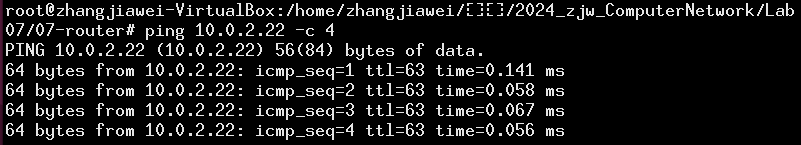
\includegraphics[width=0.8\textwidth]{h1pingh2.png}}
    \subfigure[h1 ping h3]{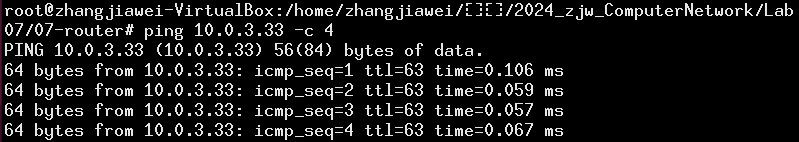
\includegraphics[width=0.8\textwidth]{h1pingh3.png}}
\end{figure}

\begin{figure}
    \centering
    \setcounter{subfigure}{2}
    \subfigure[h1 ping r1]{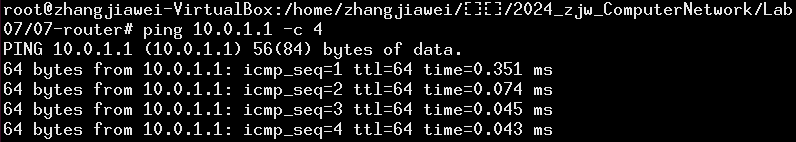
\includegraphics[width=0.8\textwidth]{h1pingr1.png}}
    \subfigure[h1 ping unreachble1]{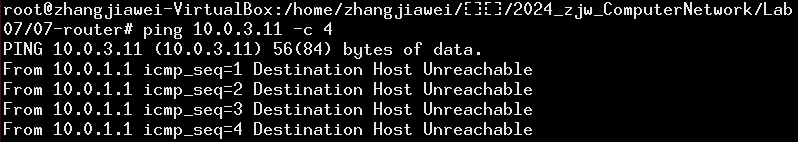
\includegraphics[width=0.8\textwidth]{h1pingun_1.png}}
    \subfigure[h1 ping unreachble2]{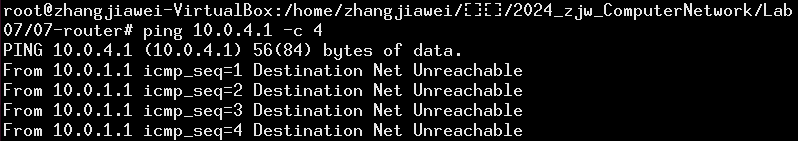
\includegraphics[width=0.8\textwidth]{h1pingun_2.png}}
    \caption{给定网络拓扑实验结果}
\end{figure}

可见,h1能够ping通h2、h3和r1,但无法ping通其他主机,说明实验结果符合预期。

\subsection{自定义网络拓扑}

自定义网络拓扑如下:

\begin{lstlisting}[language=python]
    h1, h2, r1, r2, r3 = net.get('h1', 'h2', 'r1', 'r2', 'r3')

    # 配置 IP 地址
    h1.cmd('ifconfig h1-eth0 10.0.1.1/24')
    h2.cmd('ifconfig h2-eth0 10.0.4.1/24')

    r1.cmd('ifconfig r1-eth0 10.0.1.2/24')
    r1.cmd('ifconfig r1-eth1 10.0.2.1/24')
    
    r2.cmd('ifconfig r2-eth0 10.0.2.2/24')
    r2.cmd('ifconfig r2-eth1 10.0.3.1/24')
    
    r3.cmd('ifconfig r3-eth0 10.0.3.2/24')
    r3.cmd('ifconfig r3-eth1 10.0.4.2/24')

    # 配置路由表
    h1.cmd('route add default gw 10.0.1.2')
    h2.cmd('route add default gw 10.0.4.2')

    r1.cmd('route add -net 10.0.3.0 netmask 255.255.255.0 gw 10.0.2.2 dev r1-eth1')
    r1.cmd('route add -net 10.0.4.0 netmask 255.255.255.0 gw 10.0.2.2 dev r1-eth1')

    r2.cmd('route add -net 10.0.1.0 netmask 255.255.255.0 gw 10.0.2.1 dev r2-eth0')
    r2.cmd('route add -net 10.0.4.0 netmask 255.255.255.0 gw 10.0.3.2 dev r2-eth1')

    r3.cmd('route add -net 10.0.1.0 netmask 255.255.255.0 gw 10.0.3.1 dev r3-eth0')
    r3.cmd('route add -net 10.0.2.0 netmask 255.255.255.0 gw 10.0.3.1 dev r3-eth0')

    # 执行脚本以禁用某些功能
    for n in (h1, h2, r1, r2, r3):
        n.cmd('./scripts/disable_offloading.sh')
        n.cmd('./scripts/disable_ipv6.sh')

    for r in (r1, r2, r3):
        n.cmd('./scripts/disable_arp.sh')
        n.cmd('./scripts/disable_icmp.sh')
        n.cmd('./scripts/disable_ip_forward.sh')
        n.cmd('./scripts/disable_ipv6.sh')
\end{lstlisting}

实验结果如下:

\begin{figure}[H]
    \centering
    \subfigure[h2 ping r1]{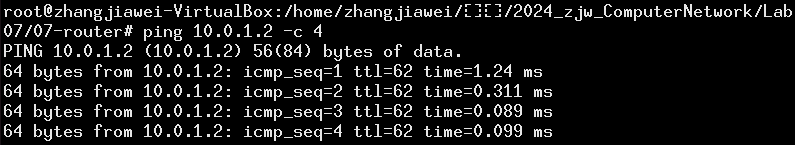
\includegraphics[width=0.8\textwidth]{h2pingr1.png}}
    \subfigure[h2 ping r2]{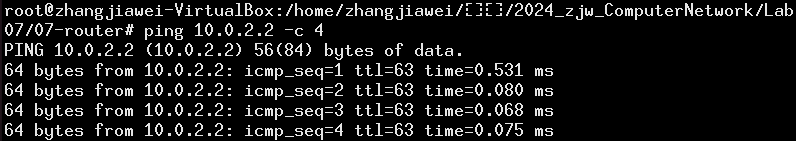
\includegraphics[width=0.8\textwidth]{h2pingr2.png}}
    \caption{自定义网络拓扑ping实验结果}
\end{figure}

\begin{figure}[H]
    \centering
    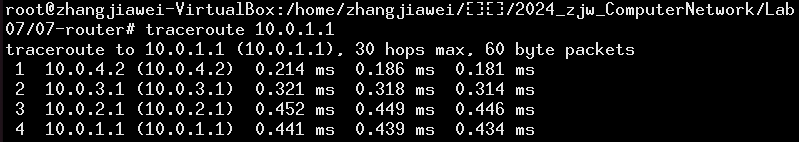
\includegraphics[width=0.8\textwidth]{h2routeh1.png}
    \caption{自定义网络拓扑traceroute实验结果}
\end{figure}

可见,h2能够ping通r1和r2,traceroute也能够正确输出路径上每个节点的IP信息,说明实验结果符合预期。

\section{实验总结}

这是一次任务量较大的实验,但同时也是一次收获颇丰的实验。通过本次实验,我学会了如何处理ARP数据包、IP数据包和ICMP数据包,实现了路由器的基本功能。在实验过程中,我对路由表的查找、ARP缓存的管理、ICMP数据包的构造和发送等方面有了更深入的了解,对网络协议栈的实现有了更深刻的认识。同时,我也学会了如何构建自定义网络拓扑,进行ping和traceroute实验,对网络通信有了更深入的了解。
\end{document}